\documentclass[a4paper,10pt]{article}

\usepackage[brazilian]{babel}
\usepackage[utf8]{inputenc}
\usepackage[T1]{fontenc}
\usepackage{titlesec}
\usepackage{graphicx}
\usepackage{mathtools}
\usepackage{amsthm}
\usepackage{amsfonts}
\usepackage[top=1.0in,bottom=1.0in]{geometry}
\usepackage{hyperref}
\usepackage[singlelinecheck=false]{caption}
\usepackage[backend=biber,url=true,doi=true,eprint=false]{biblatex}
\usepackage{enumitem}
\usepackage[x11names, rgb]{xcolor}
\usepackage{tikz}
\usetikzlibrary{snakes,arrows,shapes}

\addbibresource{../common/references.bib}

\newcommand\blfootnote[1]{%
  \begingroup
  \renewcommand\thefootnote{}\footnote{#1}%
  \addtocounter{footnote}{-1}%
  \endgroup
}

\newcommand\defeq{\mathrel{\overset{\makebox[0pt]{\mbox{\normalfont\tiny\sffamily def}}}{=}}}

\titleformat{\section}
  {\normalfont\scshape\bfseries}{\thesection}{1em}{}
\titleformat{\subsection}
  {\normalfont\scshape\bfseries}{\thesubsection}{1em}{}
\titleformat{\paragraph}
  {\normalfont}{\theparagraph}{1em}{}
\titleformat{\subparagraph}
  {\normalfont}{\thesubparagraph}{1em}{}

\captionsetup[table]{labelsep=space}

\theoremstyle{plain}

\newtheorem*{spn-def}{Definição}
\newtheorem*{spn-thm}{Teorema}

\title{\textbf{Modeling and Reasoning with Bayesian Networks: Inference with Local Structure 13.1-13.3}}

\begin{document}
\date{}
\author{}
\vspace*{-40pt}
{\let\newpage\relax\maketitle}

Relatório semana 8 - MAC0215 (Atividade Curricular em Pesquisa)

Aluno: Renato Lui Geh (Bacharelado em Ciência da Computação)

Orientador: Denis Deratani Mauá

\section{Atividades realizadas na semana}

\paragraph{
  Durante a semana foi feito um resumo dos seguintes tópicos do livro \textit{Modeling and Reasoning with
  Bayesian Networks}\cite{bayes-net-darwiche}:
}

\begin{description}
  \item[13] - Inference with Local Structure
    \begin{description}
      \item[13.1] - Introduction
      \item[13.2] - The impact of local structure on inference complexity
        \begin{description}
          \item[13.2.1] - Context-specific independence
          \item[13.2.2] - Determinism
          \item[13.2.3] - Evidence
          \item[13.2.4] - Exposing local structure
        \end{description}
      \item[13.3] - CNF encodings with local structure
        \begin{description}
          \item[13.3.1] - Encoding network structure
        \end{description}
    \end{description}
\end{description}

\section{Definição das atividades}

\paragraph{
  Foram estudadas as vantagens de se fazer inferência por estrutura local (\textit{local structure})
  explorando algumas propriedades dos parâmetros da rede, ao invés de algoritmos baseados em
  estruturas (\textit{structure-based}) como vistos nos relatórios anteriores\cite{report-2}
  \cite{report-5}.
}

\paragraph{
  Neste relatório vamos definir algumas propriedades de se fazer inferência por estrutura local e
  explicar o porquê de, em alguns casos, local structure ser melhor que structure-based. Vamos
  separar o relatório nos seguintes tópicos:
}

\begin{enumerate}
  \item Estrutura local e baseado em estrutura
  \item Impacto de estrutura local na complexidade da inferência
  \item Independência contexto-específica
  \item Determinismo
  \item Evidência
\end{enumerate}

\subsection{Estrutura local e baseado em estrutura}

\paragraph{
  Nos relatorios anteriores vimos que podemos tornar a Rede Bayesiana mais simples fazendo
  transformações na rede de tal forma que tornamos inferência mais  tratável. No entanto, tais
  algoritmos são exponenciais em tempo e espaço à \textit{treewidth}\cite{report-5} da rede. Além
  disso, esses algoritmos tentam melhorar a performance da rede pela estrutura da rede sem tomar em
  conta os valores dos parâmetros. Elas são, portanto, chamadas de algoritmos baseados em estrutura
  (\textit{structure-based}).
}

\paragraph{
  No entanto, podemos melhorar a eficiência dos algoritmos de inferência se manipularmos a rede
  levando em conta os valores específicos dos parâmetros da rede. As propriedades dos parâmetros
  da rede que permitem tal manipulação são conhecidas como paramétrica (\textit{parametric}) ou
  estrutura local (\textit{local structure}). Esse tipo de estrutura normalmente se manifestam em
  redes que envolvem restrições lógicas (\textit{logical constraints}), independência
  contexto-específica ou modelos locais de interação.
}

\subsection{Impacto de estrutura local na complexidade da inferência}

\paragraph{
  Podemos simplificar uma Rede Bayesiana paramétricamente ao compilarmos a rede e então analisarmos
  os parâmetros do circuito resultante. Por exemplo, se um circuito tiver parâmetros zero, podemos
  reduzir bastante o tamanho do circuito, assim como se um circuito possuir parâmetros distintos
  com valores iguais.
}

\paragraph{
  Além disso, considere que tenhamos uma rede tal que os nós pais de $Y$, denominados de
  $X_1,...,X_n$, formam uma relação de ou-lógico com $Y$. Adicionalmente, suponha que toda
  variável possua um valor em $\{0,1\}$ e que as variáveis $X_i$ têm distribuição normal. Ou seja:
}

\begin{enumerate}
  \item $y=1 \text{ e } x_i=1 \text{ para algum $x_i$, ou}$
  \item $y=0 \text{ e } x_i=0 \text{ para todo $x_i$.}$
\end{enumerate}

\paragraph{
  Então podemos ver que $\theta_{y|x_1,...,x_n}=1$ se e somente se obedecermos (1) ou (2).
}

\paragraph{
  Além disso, a treewidth desta rede é $n$, o que torna inferência em structure-based intratável se
  $n$ for grande o suficiente. No entanto, podemos fatorar a \textit{network polynomial}
  \cite{report-1} de tal forma que tenhamos uma polynomial representável por um circuito aritmético
  \cite{report-1} de tamanho $O(n)$, mesmo que a rede por trás tenha uma treewidth $n$. Portanto,
  podemos fazer inferência em tempo e espaço de forma linear em treewidth $n$ devido aos valores
  específicos dos parâmetros da rede.
}

\subsection{Independência contexto-específica}

\paragraph{
  A rede anteriormente discutida é um exemplo de tipo de local-structure chamada de independência
  contexto-específica (\textit{context-specific independence}). Particularmente, se um nó $X_i$ tem
  valor 1, a probabilidade de $Y$ se tornar independente dos outros nós pais $X_j$ para todo
  $j \neq i$ é:
}

\begin{equation}
  Pr(Y|x_i=1) = Pr(Y|x_1,...,x_{i-1},x_i=1,x_{i+1},...,x_n)
\end{equation}

\paragraph{
  Para todo valor $x_1,...,x_{i-1},x_{i+1},...,x_n$. Esse tipo de independência é chamada de
  context-specific pois tal independência não se mantém para certos valores de $X_i$, ou seja, se
  o valor de $X_i$ for 0, a independência não se manteria. Context-specific independence é portanto
  uma função dos parâmetros da rede, e portanto podem ser perdidas se mudarmos o valor dos
  parâmetros.
}

\subsection{Determinismo}

\paragraph{
  Considere a rede da Figura 1, composta de $n \times n$ nós binários. A treewidth dessa rede
  cresce linearmente em $n$, mas se assumirmos que cada nó assume uma função Booleana nos nós pais,
  então podemos descrever um circuito aritmético de tamanho $O(n^2)$ para essa rede, já que
  escolhendo um valor para o nó $I$ garante a implicação do valor de todo outro nó na rede.
  Portanto o número de termos não-desvanecentes (\textit{nonvanishing terms}) na polynomial network
  precisa ser igual ao número de valores para o nó $I$ e cada termo tem tamanho $O(n^2)$. A
  polynomial network terá então dois termos de tamanho $O(n^2)$ cada.
}

\begin{figure}[h]
  \centering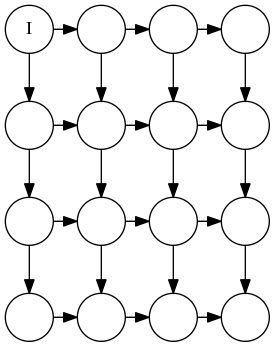
\includegraphics[scale=0.5]{imgs/grid.png}
  \caption{Uma Rede Bayesiana com estrutura em grade com $n^2$ nós. A treewidth dessa classe de
  rede cresce linearmente em $n$.}
\end{figure}

\paragraph {
  Vamos definir de forma mais geral o exemplo acima. Considere Redes Bayesianas onde cada nó
  não-raíz é funcionalmente determinada pelos seus pais, ou seja, para cada nó $X$ com pais
  $U \neq \emptyset$, temos que $Pr(x|\mathbf{u})=1$ para cada instância pai $\mathbf{u}$ e algum
  valor $x$. Isso quer dizer que $Pr(x'|\mathbf{u})=0$ para todo outro valor $x' \neq x$ e,
  portanto o valor $\mathbf{u}$ dos pais $\mathbf{U}$ implica o valor $x$ do nó filho $X$. Para
  essas redes, chamadas de redes funcionais (\textit{functional networks}), o número de
  nonvanishing terms na network polynomial é exponencial somente no número de raízes da rede,
  independentemente da treewidth.
}

\paragraph{
  Determinismo é um tipo mais geral de local structure onde parâmetros da rede tem valor zero.
  Functional networks exibem um tipo forte de determinismo, porém tal forma de local structure
  ocorre mesmo quando um nó não é funcionalmente determinado pelos seus nós pais. Seja uma variável
  $X$, por exemplo, ela pode não ser funcionalmente determinada pelos seus pais $\mathbf{U}$, porém
  um de seus valores $x$ pode ser impossível dada uma instância de seus pais $\mathbf{u}$,
  $\theta_{x|\mathbf{u}}=0$. Tal impossibilidade é chamada de restrição lógica (\textit{logical
  constraint}) e pode reduzir bastante a complexidade da inferência mesmo que não correspondam a
  dependência funcional.
}

\subsection{Evidência}

\paragraph{
  Local structure é especialmente eficaz dadas certas evidências. Considere a rede na Figura 2 (a)
  como exemplo e assuma que cada nó $S_i$ é o ou-lógico de seus pais. Supondo que a evidência dada
  é $S_1=false$, $S_2=true$ e $S_2=true$. Como $S_1$ é falso e dados pais $D_1$, $D_2$ e $D_3$,
  temos que todos esses pais devem ser também $false$. Usando o corte anteriormente visto
  \cite{report-5}, podemos aparar todas as arestas que partem destes nós, resultando na Figura 2
  (b). Note que apesar de termos visto corte de uma rede como uma técnica structure-based, devido
  à estrutura local dada pela evidência e a relação de parentesco entre os nós, pudemos aplicar
  o corte à rede.
}

\begin{figure}[h]
  \centering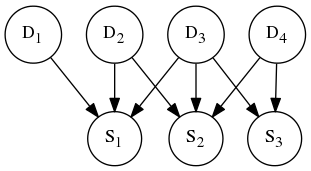
\includegraphics[scale=0.4]{imgs/evidence_a.png}
  \quad \quad \quad \quad \quad \quad
  \centering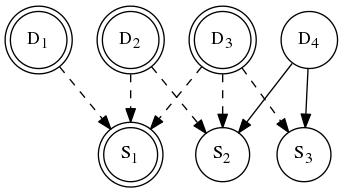
\includegraphics[scale=0.4]{imgs/evidence_b.png}
  \caption{Na esquerda (a) a Rede Bayesiana onde cada nó folha é um ou-lógico de seus pais.
    Na direita (b) vemos o resultado do corte\cite{report-5} (arestas pontilhadas) da rede dados
    $S_1=false$, $S_2=true$ e $S_3=true$.}
\end{figure}

\newpage

\printbibliography

\end{document}
